\documentclass[lettersize,journal]{IEEEtran}
%DIF LATEXDIFF DIFFERENCE FILE
%DIF DEL ./main/main.tex                          Sat Feb 21 14:03:46 2026
%DIF ADD ./Generating_a_Control_System/main.tex   Sat Feb 21 14:03:46 2026
\usepackage{amsmath,amsfonts}
\usepackage{algorithmic}
\usepackage{algorithm}
\usepackage{array}
\usepackage[caption=false,font=normalsize,labelfont=sf,textfont=sf]{subfig}
\usepackage{textcomp}
\usepackage{stfloats}
\usepackage{url}
\usepackage{verbatim}
\usepackage{graphicx}
\usepackage{cite}
\usepackage{subcaption}
%DIF < \usepackage{subfig}
%DIF -------
\usepackage[caption=false,font=footnotesize]{subfig} %DIF > 
%DIF < \usepackage{hyperref}
\usepackage{stfloats} %DIF > 
%DIF < \hyphenation{op-tical net-works semi-conduc-tor IEEE-Xplore}
% \hyphenation{op-tical net-works semi-conduc-tor IEEE-Xplore} %DIF > 
%DIF < % updated with editorial comments 8/9/2021
%DIF PREAMBLE EXTENSION ADDED BY LATEXDIFF
%DIF UNDERLINE PREAMBLE %DIF PREAMBLE
\RequirePackage[normalem]{ulem} %DIF PREAMBLE
\RequirePackage{color}\definecolor{RED}{rgb}{1,0,0}\definecolor{BLUE}{rgb}{0,0,1} %DIF PREAMBLE
\providecommand{\DIFadd}[1]{{\protect\color{blue}\uwave{#1}}} %DIF PREAMBLE
\providecommand{\DIFdel}[1]{{\protect\color{red}\sout{#1}}} %DIF PREAMBLE
%DIF SAFE PREAMBLE %DIF PREAMBLE
\providecommand{\DIFaddbegin}{} %DIF PREAMBLE
\providecommand{\DIFaddend}{} %DIF PREAMBLE
\providecommand{\DIFdelbegin}{} %DIF PREAMBLE
\providecommand{\DIFdelend}{} %DIF PREAMBLE
\providecommand{\DIFmodbegin}{} %DIF PREAMBLE
\providecommand{\DIFmodend}{} %DIF PREAMBLE
%DIF FLOATSAFE PREAMBLE %DIF PREAMBLE
\providecommand{\DIFaddFL}[1]{\DIFadd{#1}} %DIF PREAMBLE
\providecommand{\DIFdelFL}[1]{\DIFdel{#1}} %DIF PREAMBLE
\providecommand{\DIFaddbeginFL}{} %DIF PREAMBLE
\providecommand{\DIFaddendFL}{} %DIF PREAMBLE
\providecommand{\DIFdelbeginFL}{} %DIF PREAMBLE
\providecommand{\DIFdelendFL}{} %DIF PREAMBLE
\providecommand{\DIFscaledelfig}{0.5}
%DIF HIGHLIGHTGRAPHICS PREAMBLE %DIF PREAMBLE
\RequirePackage{settobox} %DIF PREAMBLE
\RequirePackage{letltxmacro} %DIF PREAMBLE
\newsavebox{\DIFdelgraphicsbox} %DIF PREAMBLE
\newlength{\DIFdelgraphicswidth} %DIF PREAMBLE
\newlength{\DIFdelgraphicsheight} %DIF PREAMBLE
% store original definition of \includegraphics %DIF PREAMBLE
\LetLtxMacro{\DIFOincludegraphics}{\includegraphics} %DIF PREAMBLE
\providecommand{\DIFaddincludegraphics}[2][]{{\color{blue}\fbox{\DIFOincludegraphics[#1]{#2}}}} %DIF PREAMBLE
\providecommand{\DIFdelincludegraphics}[2][]{% %DIF PREAMBLE
\sbox{\DIFdelgraphicsbox}{\DIFOincludegraphics[#1]{#2}}% %DIF PREAMBLE
\settoboxwidth{\DIFdelgraphicswidth}{\DIFdelgraphicsbox} %DIF PREAMBLE
\settoboxtotalheight{\DIFdelgraphicsheight}{\DIFdelgraphicsbox} %DIF PREAMBLE
\scalebox{\DIFscaledelfig}{% %DIF PREAMBLE
\parbox[b]{\DIFdelgraphicswidth}{\usebox{\DIFdelgraphicsbox}\\[-\baselineskip] \rule{\DIFdelgraphicswidth}{0em}}\llap{\resizebox{\DIFdelgraphicswidth}{\DIFdelgraphicsheight}{% %DIF PREAMBLE
\setlength{\unitlength}{\DIFdelgraphicswidth}% %DIF PREAMBLE
\begin{picture}(1,1)% %DIF PREAMBLE
\thicklines\linethickness{2pt} %DIF PREAMBLE
{\color[rgb]{1,0,0}\put(0,0){\framebox(1,1){}}}% %DIF PREAMBLE
{\color[rgb]{1,0,0}\put(0,0){\line( 1,1){1}}}% %DIF PREAMBLE
{\color[rgb]{1,0,0}\put(0,1){\line(1,-1){1}}}% %DIF PREAMBLE
\end{picture}% %DIF PREAMBLE
}\hspace*{3pt}}} %DIF PREAMBLE
} %DIF PREAMBLE
\LetLtxMacro{\DIFOaddbegin}{\DIFaddbegin} %DIF PREAMBLE
\LetLtxMacro{\DIFOaddend}{\DIFaddend} %DIF PREAMBLE
\LetLtxMacro{\DIFOdelbegin}{\DIFdelbegin} %DIF PREAMBLE
\LetLtxMacro{\DIFOdelend}{\DIFdelend} %DIF PREAMBLE
\DeclareRobustCommand{\DIFaddbegin}{\DIFOaddbegin \let\includegraphics\DIFaddincludegraphics} %DIF PREAMBLE
\DeclareRobustCommand{\DIFaddend}{\DIFOaddend \let\includegraphics\DIFOincludegraphics} %DIF PREAMBLE
\DeclareRobustCommand{\DIFdelbegin}{\DIFOdelbegin \let\includegraphics\DIFdelincludegraphics} %DIF PREAMBLE
\DeclareRobustCommand{\DIFdelend}{\DIFOaddend \let\includegraphics\DIFOincludegraphics} %DIF PREAMBLE
\LetLtxMacro{\DIFOaddbeginFL}{\DIFaddbeginFL} %DIF PREAMBLE
\LetLtxMacro{\DIFOaddendFL}{\DIFaddendFL} %DIF PREAMBLE
\LetLtxMacro{\DIFOdelbeginFL}{\DIFdelbeginFL} %DIF PREAMBLE
\LetLtxMacro{\DIFOdelendFL}{\DIFdelendFL} %DIF PREAMBLE
\DeclareRobustCommand{\DIFaddbeginFL}{\DIFOaddbeginFL \let\includegraphics\DIFaddincludegraphics} %DIF PREAMBLE
\DeclareRobustCommand{\DIFaddendFL}{\DIFOaddendFL \let\includegraphics\DIFOincludegraphics} %DIF PREAMBLE
\DeclareRobustCommand{\DIFdelbeginFL}{\DIFOdelbeginFL \let\includegraphics\DIFdelincludegraphics} %DIF PREAMBLE
\DeclareRobustCommand{\DIFdelendFL}{\DIFOaddendFL \let\includegraphics\DIFOincludegraphics} %DIF PREAMBLE
%DIF AMSMATHULEM PREAMBLE %DIF PREAMBLE
\makeatletter %DIF PREAMBLE
\let\sout@orig\sout %DIF PREAMBLE
\renewcommand{\sout}[1]{\ifmmode\text{\sout@orig{\ensuremath{#1}}}\else\sout@orig{#1}\fi} %DIF PREAMBLE
\makeatother %DIF PREAMBLE
%DIF COLORLISTINGS PREAMBLE %DIF PREAMBLE
\RequirePackage{listings} %DIF PREAMBLE
\RequirePackage{color} %DIF PREAMBLE
\lstdefinelanguage{DIFcode}{ %DIF PREAMBLE
%DIF DIFCODE_UNDERLINE %DIF PREAMBLE
  moredelim=[il][\color{red}\sout]{\%DIF\ <\ }, %DIF PREAMBLE
  moredelim=[il][\color{blue}\uwave]{\%DIF\ >\ } %DIF PREAMBLE
} %DIF PREAMBLE
\lstdefinestyle{DIFverbatimstyle}{ %DIF PREAMBLE
	language=DIFcode, %DIF PREAMBLE
	basicstyle=\ttfamily, %DIF PREAMBLE
	columns=fullflexible, %DIF PREAMBLE
	keepspaces=true %DIF PREAMBLE
} %DIF PREAMBLE
\lstnewenvironment{DIFverbatim}[1][]{\lstset{style=DIFverbatimstyle}}{} %DIF PREAMBLE
\lstnewenvironment{DIFverbatim*}[1][]{\lstset{style=DIFverbatimstyle,showspaces=true}}{} %DIF PREAMBLE
\lstset{extendedchars=\true,inputencoding=utf8}

%DIF END PREAMBLE EXTENSION ADDED BY LATEXDIFF

\begin{document}

\title{Automated UAV Controller Synthesis via LLM-Generated \\ Control Logic and Particle Swarm Optimisation}

\maketitle

\begin{abstract}
LLM-guided evolutionary frameworks for program synthesis have demonstrated strong results across combinatorial benchmarks; however, such frameworks have not been widely explored for robotic control systems. 
This paper presents an automated framework for synthesising control logic and optimising numerical coefficients, enabling the deployment of generated controllers onto robotic platforms. 
To produce deployable controllers, the framework separates control logic synthesis from numerical parameter optimisation, with controller coefficients optimised via Particle Swarm Optimisation using a Markov Decision Process reward signal.
The resulting controllers are evaluated in a custom UAV simulation environment, validated using PX4 Software-In-The-Loop, and subsequently deployed on a physical UAV. 
Controller performance is evaluated on Lemniscate and Lissajous trajectory-tracking tasks and compared against PID with disturbance observer and Linear Quadratic Regulator baselines.
Across both trajectories, the framework-generated control law achieves improved tracking accuracy relative to the baseline controllers, with a minimum reduction in mean squared error of approximately 38\% in real-world experiments. 
These results demonstrate the feasibility of deploying automatically synthesised control logic on a physical UAV, bridging automated program synthesis and real-world control deployment.
\end{abstract}

\begin{keywords}
Large Language Models, Optimisation, Control, Unmanned Aerial Vehicles
\end{keywords}

\section{Introduction}
\IEEEPARstart{D}{esign} and testing of high-performance control systems for Unmanned Aerial Vehicles (UAVs) is a difficult and time-consuming process that relies on expert knowledge.
\DIFdelbegin \DIFdel{While classical }\DIFdelend \DIFaddbegin \DIFadd{Within UAVs, }\DIFaddend control systems such as Proportional-Integral-Derivative (PID) and Linear Quadratic Regulator (LQR) remain widely used\DIFdelbegin \DIFdel{, their }\DIFdelend \DIFaddbegin \DIFadd{.
Unfortunately, PID and LQR }\DIFaddend performance is sensitive to modelling inaccuracies, parameter selection, and operating conditions.
More recently, \DIFdelbegin \DIFdel{reinforcement learning }\DIFdelend \DIFaddbegin \DIFadd{Reinforcement Learning }\DIFaddend (RL) methods have shown promise in \DIFdelbegin \DIFdel{automating controller design }\DIFdelend \DIFaddbegin \DIFadd{UAV controller design \mbox{%DIFAUXCMD
\cite{kaufmann2023champion}}\hskip0pt%DIFAUXCMD
}\DIFaddend ; however, their reliance on training data and the sim-to-real gap continue to limit their widespread adoption\DIFdelbegin \DIFdel{in real-world systems}\DIFdelend .

In parallel, Large Language Models (LLMs) have emerged as powerful tools used for much more than \DIFdelbegin \DIFdel{simple question and answer }\DIFdelend chatbots \cite{10948476}. LLMs are now being utilised for program synthesis and optimisation across a wide range of domains \cite{10937266}. Recent work has demonstrated that LLMs can generate functional code, assist local search, and even outperform human-designed heuristics in combinatorial tasks \cite{romera2024mathematical}.
Despite this progress, the application of LLMs to \DIFaddbegin \DIFadd{UAV }\DIFaddend control system synthesis remains unexplored, with little evidence that LLM-generated algorithms can be deployed on physical systems.
Key challenges include the appropriate selection of program parameters, evaluation of control systems under model mismatch, and the transition from simulation to real-world execution.

This work addresses these challenges by proposing \DIFdelbegin \DIFdel{an automated }\DIFdelend \DIFaddbegin \DIFadd{a }\DIFaddend framework that combines LLM-based program synthesis with classical optimisation and real-world \DIFdelbegin \DIFdel{validation}\DIFdelend \DIFaddbegin \DIFadd{deployment}\DIFaddend . Rather than relying on LLMs to optimise \DIFdelbegin \DIFdel{continous }\DIFdelend \DIFaddbegin \DIFadd{continuos }\DIFaddend parameters directly, we deliberately decouple controller structure from parameter tuning.
In \DIFdelbegin \DIFdel{the proposed }\DIFdelend \DIFaddbegin \DIFadd{our }\DIFaddend approach, LLMs \DIFdelbegin \DIFdel{are responsible for generating control logic, while real-valued coefficients are optimised using }\DIFdelend \DIFaddbegin \DIFadd{propose a control system for a UAV and any coefficients within that program are optimised via }\DIFaddend Particle Swarm Optimisation (PSO).
This separation \DIFaddbegin \DIFadd{of responsibilities }\DIFaddend closely aligns with established practises within Symbolic Regression (SR) and evolutionary control \DIFdelbegin \DIFdel{, enabling each component to operate within its own}\DIFdelend \DIFaddbegin \DIFadd{- using each component for its own' }\DIFaddend strengths.

Controller designs are refined through a multi-shot evolutionary querying strategy.
Previous controller programs and their performance metrics are incorporated into subsequent LLM queries, enabling \DIFdelbegin \DIFdel{a guided }\DIFdelend \DIFaddbegin \DIFadd{an }\DIFaddend optimisation procedure with quantitive feedback.
An actor-critic LLM loop is employed, whereby one model proposes control logic and another provides recommendations based on results.

The proposed framework is evaluated on a thrust-and-torque \DIFdelbegin \DIFdel{quadcopter }\DIFdelend \DIFaddbegin \DIFadd{UAV }\DIFaddend control problem.
Controllers are trained in a custom UAV environment, validated in PX4 SITL, and finally deployed onto a real UAV.
Performance is assessed on two \DIFdelbegin \DIFdel{challenging }\DIFdelend trajectory-tracking tasks and compared against a PID+DOB and LQR controller. 
The results demonstrate that the \DIFaddbegin \DIFadd{LLM-}\DIFaddend generated control system achieves superior tracking and robustness across \DIFaddbegin \DIFadd{simulated and }\DIFaddend real-world \DIFdelbegin \DIFdel{and simulated }\DIFdelend experiments.

The primary contribution of our paper is the deployment of \DIFdelbegin \DIFdel{a generated }\DIFdelend \DIFaddbegin \DIFadd{an LLM-generated }\DIFaddend control system to a UAV. Our results position LLM-assisted controller design as a viable and scalable tool for engineering applications, bridging the gap between \DIFdelbegin \DIFdel{automated }\DIFdelend \DIFaddbegin \DIFadd{UAV }\DIFaddend controller design and real-world deployment.
\section{Related \DIFdelbegin \DIFdel{papers}\DIFdelend \DIFaddbegin \DIFadd{works}\DIFaddend }
The problem this work focuses on solving is the deployment of generated algorithms in \DIFdelbegin \DIFdel{the real world}\DIFdelend \DIFaddbegin \DIFadd{to a robotic control system}\DIFaddend .
The current technical issues faced when trying to implement such a solution are related to the choice of the parameters for a given computer program, and scoring the quality of the produced computer programs within the simulation due to model mismatch.
Our specific contributions, to that end, are: multi-shot local policy search, training and test environments, and a method that utilises a UAV platform to test generated control algorithms.


\DIFdelbegin \DIFdel{In the literature, the most related paper to our work appears to be `LLM-Assisted Local Search for Policy Synthesis' \mbox{%DIFAUXCMD
\cite{sadmine2024language}}\hskip0pt%DIFAUXCMD
.
With Sadamine, Baier, and Lelis's work, they demonstrate how LLMs can be used to create programmatic }\DIFdelend \DIFaddbegin \DIFadd{Using LLM-assisted local search for policy synthesis, it is possible to create programmtic }\DIFaddend policies for various tasks \DIFaddbegin \DIFadd{with}\DIFaddend in a single shot. Notably, \DIFdelbegin \DIFdel{our work differs from theirs in two separate instances: our policies are tested in }\DIFdelend \DIFaddbegin \DIFadd{these works are not tested within }\DIFaddend the real world, and \DIFdelbegin \DIFdel{we focus on multiple queries to the LLM for program synthesis. Based on our previous work, it appears that a wide approach to program synthesis has provided better results than a small initial population for performing the local search .
}%DIFDELCMD < 

%DIFDELCMD < %%%
\DIFdel{In terms of evolutionary papers related to ours, the basis for this paper is FunSearch \mbox{%DIFAUXCMD
\cite{romera2024mathematical}}\hskip0pt%DIFAUXCMD
. Within FunSearch, the authors demonstrated how evolutionary queries can be utilised to }\DIFdelend \DIFaddbegin \DIFadd{only contain singular queries \mbox{%DIFAUXCMD
\cite{sadmine2024language}}\hskip0pt%DIFAUXCMD
. FunSearch furthers LLM-assisted local search by performing GA-like operations across generated policies \mbox{%DIFAUXCMD
\cite{romera2024mathematical}}\hskip0pt%DIFAUXCMD
. Using GA-like evolutionary techniques showcases how LLM-assisted evolutionary searching can produce heuristics that }\DIFaddend surpass human performance\DIFdelbegin \DIFdel{on combinatorial problems.
Compared to our work, which focuses on both evolutionary and local parameterisation, the FunSearch method is costly and yields significantly worse results.
The primary reasons behind the increased cost of FunSearch are related to local parameterisation.
It is unlikely that the FunSearch technique, on its own, can be used to create a high-quality control system within a reasonable time or without incurring significant excess computational cost. The inefficiencies of FunSearch are due to the choice of coefficient values within program synthesis. Opposed to simply altering a variable value, the FunSearch technique typically opts for a more complex solution to a problem.
}\DIFdelend \DIFaddbegin \DIFadd{.
}\DIFaddend 

\DIFdelbegin \DIFdel{Li et al.\mbox{%DIFAUXCMD
\cite{li2024guiding} }\hskip0pt%DIFAUXCMD
focused on an enumerative search technique for program synthesis.
Li et al.'s work focuses primarily on the synthesis of programs for solving a complex dataset (SyGuS), with a continuous bi-directional communication feedback loop for failed programs.
The primary contribution of their research is the creation }\DIFdelend \DIFaddbegin \DIFadd{Implementing an actor-critic loop within evolutionary search is shown to increase the quality of programs as solutions for complex datasets - via the usage }\DIFaddend of a `probabilistic Context-Free Grammar\DIFdelbegin \DIFdel{(pCFG)' , a list of failed programs, to help the LLM achieve a correct solution. A similar technique is used in our methodology.
Opposed to giving a specific name to this technique, we define how and why we implemented it.
For our work, we instead focus on the implicit information provided to the LLM through evolutionary queries and epigenetic program selection.
Our evolution queries include previous examples of programs, along with a meta-heuristic, the `score' of a program.
Theoretically, providing the programs in the query as our approach, as opposed to theirs, provides increased context for the model to make intelligent decisions.
Our work, rather than focusing on achieving a broad application of the technique, aims to apply the optimisation to a single use case.
This allows us to incorporate information easily and include meta-heuristic information into our queries—a difficult task to achieve in the broad sense.
}\DIFdelend \DIFaddbegin \DIFadd{' \mbox{%DIFAUXCMD
\cite{li2024guiding}}\hskip0pt%DIFAUXCMD
. It is also possible to improve the quality of critiquing within solutions by introducing multi-modality \mbox{%DIFAUXCMD
\cite{huang2025multimodal}}\hskip0pt%DIFAUXCMD
, however, due to cost constraints this technique is not used within our work.
}\DIFaddend 

\DIFdelbegin \DIFdel{A related work that might help support the theoretical results of this approach, which has not been implemented, is the usage of multimodality within query generation before program synthesis.
For example, Huang et al. \mbox{%DIFAUXCMD
\cite{huang2024multimodal} }\hskip0pt%DIFAUXCMD
performed work utilising GPT-4's multimodal features, demonstrating how multimodality can enhance optimisation performance.
In the context of our work, implementing this makes sense simply due to the ease and clarity with which information about a trajectory can be displayed in a visual format.
However, a decision was made not to incorporate multimodal queries within our results, primarily due to our incentive to keep the monetary cost of generation at zero.
We believe that ensuring the optimisation process is free increases much-appreciated scrutiny and facilitates widespread adoption.
}%DIFDELCMD < 

%DIFDELCMD < %%%
\DIFdelend For a recent review and survey of papers covering the relevant topic area, the authors recommend either Wu et al. \cite{wu2024evolutionary} or Huang et al. \cite{huang2024large}. Both papers provide a comprehensive overview of the current progress in Large Language Models and Optimisation.

\DIFdelbegin \DIFdel{The reasoning behind this decision is that PSO has proven effective on a range of control problems. For example, researchers have applied PSO to automatically tune PIDgains for UAV attitude and position control , achieving improved trajectory tracking performance without manual tuning \mbox{%DIFAUXCMD
\cite{rinaldi2025pso}}\hskip0pt%DIFAUXCMD
. }\DIFdelend \DIFaddbegin \DIFadd{UAV control is largely dominated by four main control systems: PID \mbox{%DIFAUXCMD
\cite{sahrir2022modelling}}\hskip0pt%DIFAUXCMD
, Reinforcement Learning \mbox{%DIFAUXCMD
\cite{kaufmann2023champion}}\hskip0pt%DIFAUXCMD
, MPC \mbox{%DIFAUXCMD
\cite{ganga2017mpc}}\hskip0pt%DIFAUXCMD
, and non-predictive model-based methods \mbox{%DIFAUXCMD
\cite{masse2018modeling}}\hskip0pt%DIFAUXCMD
. PID controller remain the dominant control system, due to ease of use. The issues with PID are the requirement for tuning for optimal performance. RL is currently the optimal technique, however relies on extensive model building and environmental data. MPC has the same drawbacks as RL, however it also requires a lot of compute during runtime to compute optimal trajectories. Finally, LQR based method are focused on the drawbacks of PID, making tuning easier. The problem with LQR is the requirement for an algebraic equation to be solved for optimal control each timestep, and the expertise required to implement the model for the control system.
}\DIFaddend 

\DIFdelbegin \DIFdel{To our knowledge, no one has yet deployed a generated algorithm in the real world.
}\DIFdelend \DIFaddbegin \DIFadd{Evolutionary robotics and GP-based techniques have been investigated for control system usage, usually parametrised via neural or symbolic structures \mbox{%DIFAUXCMD
\cite{kala2012multi}}\hskip0pt%DIFAUXCMD
. Our work instead focuses on tractable LLM-generated control laws.
}\DIFaddend 

\DIFaddbegin \DIFadd{Unlike optimal control formulations that assume known model structure and quadratic costs \mbox{%DIFAUXCMD
\cite{masse2018modeling}}\hskip0pt%DIFAUXCMD
, this work automates the synthesis of the control structure itself.
}\DIFaddend \section{Methodology}
\DIFaddbegin \label{sec:method}
\DIFaddend % Our approach to the LLM-driven optimisation framework begins with a dual-query method to instruct and guide the LLM towards optimal programs.
% We phrase these dual-query parts as the static part, which never changes, and the dynamic part.
% Definition of the problem, specific implementation details, return values, and function parameters are considered to be static query aspects and never change through program evolution.
% Contrary to the static query, the dynamic part describes actionable insights and useful information about the function.
% The dynamic query part also contains previous exponentially sampled (from the program history) examples of functions and their related scores.
% Changes to the dynamic part of the query are made each iteration through a secondary LLM in an agentic fashion.
% Both primary and secondary LLMs collabarte towards the solution, with the primiary LLM offering code-based solutions and the secondary LLM providing recommendations.
% During each population round, the secondary LLM is queried to help describe the newly generated function, and its output appended to the dynamic query.
% This could be viewed as a `tutor` and `student`, or `actor-critic` LLM collaboration, whereby the tutor/critic recommends improvements, the student/actor implemenents these improvements, then reports back progress \& score to the tutor/critic.
Our approach employs a dual-query Large Language Model (LLM) framework to automatically synthesise a thrust/torque UAV controller.
A primary critic LLM first generates a high-level specification for a controller, and a secondary critic LLM analyses simulation responses and suggests feedback.
Collaboration between the actor and critic forms an actor-critic LLM loop, motivated by successes in LLM-assisted program synthesis \cite{luo2024large}.
LLMs can produce functional code for most tasks, but pairing with a critic or verification step improves reliability \DIFdelbegin \DIFdel{\mbox{%DIFAUXCMD
\cite{wang2025multi}}\hskip0pt%DIFAUXCMD
}\DIFdelend \DIFaddbegin \DIFadd{\mbox{%DIFAUXCMD
\cite{le2024indict}}\hskip0pt%DIFAUXCMD
}\DIFaddend .
When implemented in this manner, the LLM is proposed to refine its output based on performance, which is synonymous with self-reflection and In-Context-Learning (ICL) \DIFdelbegin \DIFdel{\mbox{%DIFAUXCMD
\cite{dong2022survey}}\hskip0pt%DIFAUXCMD
}\DIFdelend \DIFaddbegin \DIFadd{\mbox{%DIFAUXCMD
\cite{dong2024survey}}\hskip0pt%DIFAUXCMD
}\DIFaddend .
By incorporating a critic model, we improve performance, similar to recent LLM approaches that use an agent to verify actions \DIFdelbegin \DIFdel{\mbox{%DIFAUXCMD
\cite{wang2025multi}}\hskip0pt%DIFAUXCMD
}\DIFdelend \DIFaddbegin \DIFadd{\mbox{%DIFAUXCMD
\cite{le2024indict}}\hskip0pt%DIFAUXCMD
}\DIFaddend .
The two LLMs operate together: the primary LLM proposes a control logic structure, and the secondary LLM implements the logic and provides quantitative feedback.

A key and deliberate feature of our method is the abstraction of code logic and the optimisation of numerical coefficients. The LLM pair performs high-level decision making and program synthesis (e.g., controller design, conditional logic), with the real-valued coefficients (e.g., vehicle mass and controller gains) of the program optimised via classical methods. The reasoning behind this deliberate abstraction is simple: LLMs excel at writing structured code from descriptions and making high-level decisions, yet lack direct real-value optimisation capability. Our approach mirrors that of Symbolic Regression, whereby a genetic programming technique evolves a high-level topology, with classical optimisers tuning constants \cite{cranmer2023interpretable}. Similarly, our approach produces a human-readable control policy, with placeholder values treated as tunable parameters. This separation of responsibilities is advantageous as it combines expert knowledge ingested by LLMs during training with the search capabilities of optimisation for real-valued parameters. We refer to this separation of duties as program specification (controller design) and program parameterisation (optimisation of parameters).

To implement the program parameterisation stage, we use Particle Swarm Optimisation (PSO). In our specific case, each particle represents a set of program coefficients (e.g., PID gains). The PSO algorithm optimises the coefficients to minimise the trajectory-tracking error for a given program. The simulated fitness score enables the PSO algorithm to converge towards a suitable parameter set for each controller. We modified the standard PSO algorithm to enhance the global stability criteria for our problem.

Firstly, the inertia decays over time, resulting in exploitation of the search space nearer the end of the search \cite{shi1999empirical}:
\begin{equation}
    \omega(t) = \omega_{\text{max}} - \left( \frac{\omega_{\text{max}} - \omega_{\text{min}}}{T} \right) t
\end{equation}
with $\omega_{\text{max}}$ and $\omega_{\text{min}}$ representing the maximum and minimum inertia, \DIFdelbegin \DIFdel{and }\DIFdelend $T$ representing the total number of iterations\DIFaddbegin \DIFadd{, and $t$ representing the current timestep}\DIFaddend .

Time-varying acceleration coefficients for social and personal coefficients are also applied to the algorithm \cite{van2006study}:
\begin{equation}
    c_1(t) = c_{1,\text{min}} + \left( c_{1,\text{max}} - c_{1,\text{min}} \right) \frac{t}{T}
\end{equation}

\begin{equation}
    c_2(t) = c_{2,\text{max}} - \left( c_{2,\text{max}} - c_{2,\text{min}} \right) \frac{t}{T}
\end{equation}

And finally, the velocity is clamped such that particles cannot move too fast across the search space \cite{shahzad2014probabilistic}:

\begin{equation}
    PSv_{\text{max}}(t) = v_{\text{max, initial}} - \left(\frac{v_{\text{max, initial}} - v_{\text{max, final}}}{T}\right) t.
\end{equation}

To further refine the generated solution, another local search step is performed upon the optimal program before deployment and testing. We take the best solution from PSO and perform a larger optimisation step to ensure that a better set of coefficients has not been missed. That is, a course initial optimisation is performed, followed by a finer second optimisation on the best-scoring program. The justification for this step stems from analyses of PSO, which indicate that PSO converges to local optima without guaranteeing global optimality \DIFdelbegin \DIFdel{\mbox{%DIFAUXCMD
\cite{fitas2024optimal}}\hskip0pt%DIFAUXCMD
}\DIFdelend \DIFaddbegin \DIFadd{\mbox{%DIFAUXCMD
\cite{van2010convergence}}\hskip0pt%DIFAUXCMD
}\DIFaddend . This final search exploits the best solution and fine-tunes parameters for minor performance improvements. Essentially, PSO is used in a global sense under broad search constraints, and a subsequent search is performed to refine the result. A combination of a final, deeper refinement stage with a fast-searching stage enables the finalisation of our algorithm, which identifies a near-optimal set of coefficients for the generated controller.

\subsection{Implementation pipeline}
Notably, all the steps listed below are automated, and our algorithm requires only a description of the problem and the loss function to begin optimisation. See Figure \ref{fig:full_system} for a general overview of this automated process.

We begin by querying the LLM with a detailed description of the task at hand and specific requirements. For our case, this prompt also included an example base controller (PID). It is not necessary to include a base template, as discussed in \cite{romera2024mathematical}; however, faster convergence is achieved with a given base. The prompt also includes structural and typographic information (C++, return values, frame translations). We also ensure that the prompt consists of details on placeholder coefficient gains and how to access them. The actor LLM's response produces an initial set of viable population members. For each response we receive, we ensure that it compiles without runtime or compilation errors before assuming it is a valid response. For any set of invalid responses received, the actor LLM is queried again for a new output until a complete set of admissible programs is available for testing.

The admissible set of responses is then integrated into the simulation environment to perform optimisation. We run our RVO stage to estimate each controller's performance. The final fitness for each computer program is recorded in a Table, along with the program's identification number (ID) and score. The loss function is designed so that the minimum score in the Table above corresponds to the identification number of the optimal-performing program. Any number of elite population members can be saved for the next generation and appended to the next generation's query. Realistically and pragmatically, in our algorithm, it only makes sense to keep the most elite population member.

The environment and experiments are an ad-hoc UAV simulation based on Flightmare (details of which are listed in Section \ref{subsec:simulated_training_environment}) \cite{song2020flightmare}. The environment allows us to place the LLM's output \DIFdelbegin \DIFdel{'}\DIFdelend \DIFaddbegin \DIFadd{`}\DIFaddend in-testing', enabling automated observation of behaviours with performance metrics. 

The automated metrics are provided to the critic LLM, along with the code, to integrate high-level observational critiques into the actor's control design. During this stage, multimodality could be a key feature. Providing a visual demonstration of the current optimal controller output could lead to better insights into actionable goals for the actor to implement. For example, the critic that provides information such as `the drone overshoots the target` offers much better insight into the program's performance than descriptions of performance metrics. Multimodality has not been implemented in our algorithm due to both cost constraints and scope. The critic output and observations are appended to the query for the next generation of the population, thereby providing closed-loop feedback. This collaborative feedback loop creates an actor-critic dynamic and aligns with emergent LLM practices of using self-reflection to refine solutions.

Upon receiving the critic's response regarding program performance, we begin defining the query for the actor to produce the next generation. The new query starts again with the problem description and specific requirements, which we consider static and never change during program evolution. Exponentially sampled (based on score) examples of previous population members are included in the new query. The reasoning behind an exponential sample of the program history is based on our understanding of Epigenetic DNA, whereby previous genes are not forgotten; they are less likely to be expressed. After joining the previous examples onto our new query, we add the critic's response. This new query forms the basis for the actor's implementation of the next-generation population.

\begin{figure*}[htb]
    \centering
    \includegraphics[width=\linewidth,height=0.28\linewidth]{figures/full_system.pdf}
    \caption{\textbf{System overview: } An overview of the LLM for optimization process.}
    \label{fig:full_system}
\end{figure*}


The process is repeated until either the convergence criteria are met or the maximum number of iterations is reached. In summary, the stages are: query construction, actor program synthesis, real-valued optimisation, population selection, and critiquing. A general overview of this process is provided for easy viewing in Figure \ref{fig:full_system}.

\DIFaddbegin \DIFadd{Our custom simulation environment is designed as a Markov Decision Process (MDP) chain, which integrates UAV dynamics. It is possible to reset the simulation, view rewards, apply control actions, and retrieve observations at each timestep. This allows for easy integration with the RVO optimisation step, in which the cumulative sum of rewards serves as the loss function for each rollout, and the simulation can be reset for each particle. The simulation operates with an 8ms interval for physics updates and control loops. By framing our simulation as an MDP, we ensure reproducibility and ease of scenario configuration. All simulations were run on a 32-core computer without using a GPU. Each simulation rollout took a few seconds, so the total optimisation and testing of the generated controls took around 5 minutes per iteration.
For our full simulation, we ran for 100 generations, using a population size of 30. For the PSO parameters, we used 300 particles with 10 dimensions. For fine-tuning the final model, we used 10,000 particles across 10 dimensions.
The PSO particles were had no bounds for exploration, due to the general purpose usage of the program coefficients, however, they were initialised uniformly within the range $[-1,1]$. Particle velocity was clamped to a maximum value of 1.0, such that both large and small coefficients could be effectively explored. Dynamic social and personal weighting was in effect, discussed in Section \ref{sec:method}, however the initial value for the social $c_1$ and personal $c_2$ parameters was set to $0.5$ and $0.8$ respectively.
In total, we trained for around 30 minutes before seeing results that outperformed the baseline. The full training loop (100 iterations) took 5 hours. Exact token usage was not calculated during the training process, and requires further investigation. For the full training procedure, the cost whilst using GPT 3.5-turbo came to be £0.80 (GBP).
}

\DIFadd{For the LLM querying, GPT-3.5 turbo was used with a temperature setting of 0.6 and a top\_p value of 0.1. The context window length of GPT 3.5-turbo, 4,096 tokens, had enough space to fit both parts of the query; the static and evolutionary query parts both fit inside the context window.
}

\subsection{\DIFadd{The critic}}
\DIFadd{The critic performs an analysis of the provided control system and offers areas for improvement. Each generation, the optimal program per-island is provided to the critic for analysis. The critic determines issues with the control system and provides recommendations on areas for improvement. The critic response is appended to the primary population candidate query for the next generation. This forms a closed loop, whereby current optimal programs are critiqued, improved, and critiqued again. In our research, we used the same model (GPT-3.5-turbo) for the critic as the main program.
}

\DIFaddend \subsection{Simulated training environment}
\label{subsec:simulated_training_environment}

The equations used to describe the UAV and its movement across time are supplied by the vast research done by \cite{ijcai2021p650, faessler2017differential, faessler2017thrust, loquercio2020deep}.

 To control the UAV, we utilise mass-normalised collective thrust and body-torque ($A \in \mathbb{R}^{4}$ ) measured in Newtons. The upper bound of the collective thrust is calculated as the maximum thrust produced by all four motors, as determined by measurements. The maximum body torque is the most significant differential between any two given motors.

To simulate thrust from the given outputs, the control policy output is first converted into motor angular velocity (RPM), denoted $r_{i}^{des} \in \mathbb{R}^{4}$, the equations for which are given by
\begin{equation}
    r^{des} = I A \omega'_t + \omega' \times \left( I \omega' \right),
\end{equation}
with $A$ being the motor allocation matrix, provided as 
\begin{equation}
\[
\mathbf{A}
=
\begin{bmatrix}
1 & 1 & 1 & 1 \\[4pt]
l \sqrt{\tfrac{1}{2}} & -l \sqrt{\tfrac{1}{2}} & -l \sqrt{\tfrac{1}{2}} & l \sqrt{\tfrac{1}{2}} \\[4pt]
-l \sqrt{\tfrac{1}{2}} & -l \sqrt{\tfrac{1}{2}} & l \sqrt{\tfrac{1}{2}} & l \sqrt{\tfrac{1}{2}} \\[4pt]
k_1 & -k_2 & k_3 & -k_4
\end{bmatrix}.
\]
\end{equation}
The RPM is then passed through a first-order motor model to simulate the motor's internal dynamics,
\begin{equation}
    \dot{r_{i}} = \frac{1}{\alpha_{i}} (r^{des}_{i} - r_{i}) \label{eq:first_order_filter}
\end{equation}
% The commanded output to RPM and RPM to thrust are both measured using a motor test kit on the real motors and creating a linear relationship between the variables.
% This process aims to simulate the dynamics of the motor system and provide a more realistic representation of the achieved thrust in the UAV.
where $\alpha_{i}$ is the motor ramp time for the $ith$ rotor.

A linear model based on data from the UAV motors is used to convert the RPM of the motor into thrust:
\begin{equation}
    f_{i} = r_{i}^{2} \cdot M_{c}
    \label{eq:rpm_to_force}
\end{equation}
Where $M_{c}$ is the constant for the motor-propeller pair.
These thrust values allow the definition of a three-axis body torque matrix $\eta \in \mathbb{R}^{3}$ and collective thrust $c$:
\begin{equation}
    \eta = \begin{bmatrix} \frac{l}{\sqrt{2}}\left(f_{1} - f_{2} - f_{3} + f_{4}\right)   \\
        \frac{l}{\sqrt{2}}\left(-f_{1} - f_{2} + f_{3} + f_{4} \right) \\
        k_{1}f_{1} - k_{2}f_2{} + k_{3}f_{3} - k_{4}f_4
    \end{bmatrix}, \label{eq:three_axis_torque}            \\
\end{equation}

\begin{equation}
    c = f_{1} + f_{2} + f_{3} + f_{4}, \label{eq:collective_thrust}
\end{equation}
where $l$ is the UAVs arm length, $f_{i}$ is the thrust produced by the motors, and $k_{i}$ is the rotor drag co-efficient.


Given the filtered body torque and collective thrust, it is possible to transition between timesteps with the following equations (note Lagrange notation for derivatives):
\begin{equation}
    P'           = V
\end{equation}
\begin{equation}
    V_{wb}'      = Q_{wb} \odot c-G-RDR^{T}v
    \label{eq:velocity}
\end{equation}

\begin{equation}
    Q_{wb}'      = \frac{1}{2}\lambda(\omega_{wb}) \cdot q_{wb}
    \label{eq:quaternion}
\end{equation}
where $\lambda(\omega_{wb})$ is a skew-symmetric matrix of the vector $(0, \omega^{T})^{T} = (0, \omega_{x}, \omega_{y}, \omega_{z})^{T}$.
\begin{equation}
    \omega_{wb}' = I^{-1}\cdot (\eta-\omega_{wb}\times I\omega_{wb})
\end{equation}
where $G = [0, 0, -g]^{T}$, $R \in \mathbb{R}^{3,3}$ is a rotation matrix of the form $R = \left\{X_{b}, Y_{b}, Z_{b}\right\}$,
$D$ is a diagonal matrix defining rotor drag coefficients $D = diag(d_{x}, d_{y}, d_{z})$, $\odot$ denotes the multiplication of a vector and quaternion, and the inertia matrix $I$ of the UAV is given by $\mathbf{I} = \text{diag}\{I_{xx},I_{yy},I_{zz}\}$ in which each $I_*\in\mathbb{R}$ is the moment of inertia about each of the UAV's body-axes.

The following equation is used to estimate the UAV's inertia, which we use throughout the simulation.
\begin{equation}
    \hat I = \frac{m}{12} l^{2} D
\end{equation}

For the observation state of the policy, Brownian motion noise is added to the linear and angular velocities, simulating both a random walk and a per-timestep disturbance. The noise added to the environment is somewhat complicated to write down mathematically, so \DIFdelbegin \DIFdel{a GitHub link is provided for those who wish to view }\href{https://github.com/PX4/PX4-SITL_gazebo-classic/blob/70683dc759cbd3ebccfa78429b564f8b1fb5d149/src/gazebo_imu_plugin.cpp}{\DIFdel{here}}%DIFAUXCMD
\DIFdelend \DIFaddbegin \DIFadd{we have provided a reference for those wishing to view \mbox{%DIFAUXCMD
\cite{PX4_gazebo_imu_plugin_2023}}\hskip0pt%DIFAUXCMD
}\DIFaddend .


Each timestep, the controllers recieves a state $S = [P, \Omega, P', \Omega'], S \in \mathbb{R}^{12}$, and provides the desired body torque and collective thrust $A = [a_0, a_1, a_2, a_3], A \in \mathbb{R}^{4}$.

The values we use for our UAV are provided in Table \ref{tab:quad_model_params}

\begin{table}[h!]
\centering
\caption{Quadcopter Model Parameters}
\begin{tabular}{l l}
\hline
\textbf{Symbol} & \textbf{Value} \\
\hline
$g$ & $9.81\,\mathrm{m/s^2}$ \\
$\alpha^{-1}$ & $0.0125\,\mathrm{s}$ \\
$\Delta t_{\mathrm{sim}}$ & $0.008\,\mathrm{s}$ \\
$M_c$ & $7.84\times 10^{-6}$ \\
$k_i$ & $1.75\times 10^{-4}$ \\
$m$ & $2.0\,\mathrm{kg}$ \\
$l$ & $0.225\,\mathrm{m}$ \\
$D$ & $\mathrm{diag}(4.5,\,4.5,\,7)$ \\
\hline
\end{tabular}
\label{tab:quad_model_params}
\end{table}

All results are provided and calculated using \DIFdelbegin \DIFdel{either }\DIFdelend the Mean Squared Error (MSE) \DIFdelbegin \DIFdel{or Sum of Squared (SSE) errors. Thus, both SSE and MSE are given }\DIFdelend \DIFaddbegin \DIFadd{of positional reference error across all axis, }\DIFaddend in $m^2$ units.
\DIFdelbegin \DIFdel{These are all calculated as the mean error across all axes.
}\DIFdelend 


% Implemented in such a way, we can test the controller across various tasks using performance metrics. This step effectively places the LLM's output 'in-testing', allowing for an observation of behaviour in a virtual environment. 


% In engineering problems, it is imperative to have a correct estimation of any given model or coefficient values.
% It is difficult to dynamically provide this information to the LLM, without knowledge of what its solution will look like.
% To resolve this issue, and improve generated code performace, we make usage of a local search process across variables which are provided to the LLM.
% The static query part consists of some statements describing to the LLM that for \textit{any} usage of a co-efficient within its code, it must access them through the provided vector.
% Resultant generated code thus has no dependency upon estimating correct variable values, and is instead entirely focused on program specification.
% This is important for engineering model development, due to the LLM not having the knowledge required for specific platforms or disturbances.
% Resolution of the aforementioned problems results in code which non-model specific, allowing for catering to our specific model.



% An important aspect of using local search within LLM-driven optimisation is to describe to the LLM that it must make use of provided search variables.
% In our specific implementation, we provided to the function a set of co-efficients by the name `coefs`.
% That is, the LLM provides coefficients to use throughout the generated function.
% When creating the static part of the query, we described to the large language model that for \textit{any} usage of a coefficient within its code, it must access the variable from the coefficient array.
% The LLM, then, has no requirement for estimating correct values for variables, and is instead entirely focused on computer program synthesis - opposed to model estimation.

% After creating the querying part of the system, implementation of the GA aspect of LLM-driven optimisation follows.
% The LLM is queried \textit{N} number of times, with each query producing a new population member.
% These populations are scored according to a fitness function, and the best-performing members of the population are retained for the next iteration.
% We provide the reference location to the generated controller(s) as a position reference $p_r\in\mathbb{R}^{3\times1}$ which represents the target location in the world-fixed frame. The reference position is assumed to be smooth and continuously differentiable

% \begin{equation}
%     R^{t} = P^{t} - P_{r}^{t}.
%     \label{eq:poss_reward}
% \end{equation}

% We only use the positional reward for our training policy as the trajectory that the quadcopter must take, which fully excites system dynamics, is a time-derived function and thus incorporates velocities and rotations within by definition.

% \subsection{Testing implementation}
% \begin{figure}[!h]
%     \includegraphics[width=\textwidth]{figures/method_comparison.pdf}
%     \caption{
%     \textbf{Testing methodology: } We ran small-scale experiments to confirm some additions to the surrogate optimisation method. In the figure, `both' refers to the method with epigenetic sampling and evolutionary queries enabled, `Evol.' shows the results for evolutionary queries only, `Epig.' shows the results for epigenetic queries only, and `None' refers to baseline surrogate-assisted optimisation. }
%     \label{fig:boxplots_compare}
% \end{figure}

% In Figure \ref{fig:boxplots_compare}, we provide a summary of the changes we made to the LMEA algorithm and the relative performance increase.

% Results are gathered from the training simulator using SSE. Both achieve a final SSE of 184.354 $ m^2$, Evolutionary queries 375.946 $ m^2$, Epigenetic sampling 272.549 $ m^2$, while implementing neither technique achieved 366.748 $ m^2$.

% The postulated hypothesis for such improvement, while unsubstantiated, is that evolutionary queries allow the model to focus on single improvements per-evolution, ensuring the best implementation for each suggested improvement, and epigenetic queries allow the model to view older techniques that may provide a small benefit to the control law.

% For the ablation, we ran for 20 iterations with a population size of 30.
% Interestingly, LMEA had access to all optimisation methods within this task (as a recursive function call); however, it was still outperformed by RVOLMEA, which was itself limited by PSO.
% To implement this fast analysis of differing algorithmic changes, we used the BLADE LLM benchmarking framework \cite{van2025blade}.
% Each instance is run for five generations with a population size of 3.
% The hyperparameters of the surrogate optimisation model remain the same for each method.
% The performance of each method is benchmarked against all problems within the BBOX Experiment.
% The results presented here are the best fitness program compared to each optimisation problem, stratified by algorithm changes.


\DIFdelbegin \subsection{\DIFdel{Experiments}}
%DIFAUXCMD
\addtocounter{subsection}{-1}%DIFAUXCMD
\DIFdel{Our custom simulation environment is designed as a Markov Decision Process (MDP) chain, which integrates UAV dynamics. It is possible to reset the simulation, view rewards, apply control actions, and retrieve observations at each timestep. This allows for easy integration with the RVO optimisation step, in which the cumulative sum of rewards serves as the loss function for each rollout, and the simulation can be reset for each particle. The simulation operates with an 8ms interval for physics updates and control loops. By framing our simulation as an MDP, we ensure reproducibility and ease of scenario configuration. All simulations were run on a 32-core computer without using a GPU. Each simulation rollout took a few seconds, so the total optimisation and testing of the generated controls took around 5 minutes per iteration.
For our full simulation, we ran for 100 generations, using a population size of 30. For the PSO parameters, we used 300 particles with 10 dimensions. For fine-tuning the final model, we used 10,000 particles across 10 dimensions.
}\DIFdelend %DIF >  \subsection{Experiments}


% The simulated environment for training is framed as an MDP chain, such that Monte Carlo rollouts can be used to approximate performance.
% The inner workings of the simulated environments are designed to fit an OpenAI Gym \cite{brockman2016openai} interface.
% At each step, the environment receives an action from the control system, and then returns the next state for the control system to solve.
% The environment keeps track of an accumulated reward for the control system, which is returned as the final score for the given control system.

% During training, the agent receives as input the state $\mathcal{S} = [\textbf{P}, \omega, \textbf{V}, \omega']$ where $P$ is the distance between the body-fixed frame position and goal position, $\omega$ represents the Euler rotation angles, $V$ is the linear velocity, $\omega'$ is the angular velocity. These values are all that is known to the LLM in relation to the program state.
% We exclude acceleration from the state-observation input due to the difficulty in measuring exact accelerations on mobile systems.
% % As output the control policy must return the body-torque and collective thrust.

% Two experiments are formulated for testing the ability of LLMs to produce code for various tasks.
% In the first experiment, the control system requires that the UAV follows a full double slanted leminscate trajectory under nominal flight conditions.
% The generated trajectory is designed to excite the full system dynamics, such that a good approximation of true flight performance can be gathered from a single lap.
% The second experiment tests the ability of the technique to produce code for impulse disturbance.

\subsection{Trajectory Tracking}
The primary task for the generated controller was to accurately track an oscillating lemniscate trajectory. We chose a lemniscate as the reference position, as it is a complex trajectory to follow. The lemniscate requires the UAV to perform continuous turns in opposite directions, thereby exciting the UAV's dynamics and challenging the controller's response. We define the lemniscate trajectory as:

\begin{equation}
    P_r^t = \begin{bmatrix}
   rad\,\sin\bigl(\theta(t)\bigr),\\
   rad\,\sin\bigl(2\,\theta(t)\bigr),\\
   z_0 + \sigma(t)\,A\,\sin\bigl(\theta(t)\bigr)
   \end{bmatrix}
   \label{eq:trajectory}
\end{equation}

with $rad$ controlling the circle radius, $z_0$ controlling the height, t is the timestep multiplied by $\Delta$t, $A$ controlling the vertical offset, and $\theta(t)$ provided as

\begin{equation}
    \theta(t) = 2\pi \frac{t}{T}.
\end{equation}

Our experiment is designed so that each rollout completes in 40 seconds, yielding 10,000 simulation timesteps. As noted in prior work, lemniscate trajectories exhibit rapid, coordinated attitude changes while maintaining stability. The initial state for the quadcopter at $t=0$ is provided as some distance away from the trajectory's initial position: $P_x=1$, $P_y=-1$. Additionally, the controller starts with a large yaw offset. Implementing an initial positional offset and rotational bias allows us to estimate the controller's performance for large and small reference errors within a single simulation run. Tracking performance is evaluated using a standard metric: the Sum of Squared Error of the position coordinates
\begin{equation}
    L(\pi) = \sum_t^T (P^{t} - P_{r}^{t})^2.
\end{equation}

\subsection{Lissajous Trajectory}
The controllers are also tested on a Lissajous trajectory. The Lissajous trajectory is not observed by any controller in the training environment, ensuring that the controllers and parameters are not overfitting to any single trajectory. The Lissajous trajectory is a good choice for our Out-Of-Distribution (OOD) testing, as it provides a strong snap impulse error to the controller reference error.
\DIFdelbegin \DIFdel{Testing the controllers on two complex trajectories, each with its own difficulties, demonstrates the controllers' robustness across various trajectory types.
}\DIFdelend 

We formulate the trajectory reference as

\begin{equation}
P_r^t 
=
\begin{bmatrix}
R_x \sin\!\left(\kappa_x t\right) \\
R_y \sin\!\left(\kappa_y t + \phi_y\right) \\
A_z \sin\!\left(\kappa_z t + \phi_z\right)
\end{bmatrix}
\end{equation}
with $\kappa_x$, $\kappa_y$, and $\kappa_z$ controlling the frequency of oscilations across each axis. No starting position offset is used for the Lissajous trajectory.


% A figure of this trajectory is provided in Figure \ref{lemniscate_traj}.

% \begin{figure}[!h]
%     \centering
%     \includegraphics[width=0.5\linewidth]{fig1.png}
%     \caption{Generating lemniscate trajectory that the quadcopter must follow.}
%     \label{fig:lemniscate_traj}
% \end{figure}

% Defining our trajectory function as in \ref{eq:trajectory} allows for a large simplification of the loss function for any given control system

% Given our trajectory function incorporates time, rotation, and velocity integrated into position, we simply create a negative signal for distance from the provided position

% \subsection{Impulse rejection}
% To demonstrate the robustness of our algorithm to various problems, we conducted an impulse rejection experiment. This scenario mimics an external shock to the system, such as a gust of wind or a collision. Figure \ref{fig:ball_drop} describes the simulated experiment visually.

% \begin{figure}[!h]
%     \centering
%     \includegraphics[width=0.5\linewidth]{figures/ball drop experiment.pdf}
%     \caption{Depiction of the ball drop experiment. A ball is dropped from a set height above the UAV, with the contact point creating an angular and collective thrust disturbance. Within the simulation, $b_x$ and $b_y$ are randomised from a standard normal distribution.}
%     \label{fig:ball_drop}
% \end{figure}

% In simulation, we implement the disturbance as a large impulse applied on a single timestep. Specifically, at $t=400$, a vertical force is applied to the UAV along its body axis, and the response is measured. The task of the controller in this experiment was to reject the disturbance with minimal deviation from the hover position.

% To simulate the impulse experiment, a simplistic model is used, which samples a random contact point and applies a wrench disturbance rotated by the contact point.

% \begin{subequations}
% \begin{align}
%     ball_v &= \sqrt{2 g b_h} \\
% % \end{equation}
% % \begin{equation}
%     ball_{mag} &= 0.5 \cdot ball_v + N(0,1)\\
% % \end{equation}
% % \begin{equation}
%     b_x &\sim N(0, 1)\\
% % \end{equation}
% % \begin{equation}
%     b_y &\sim N(0, 1)\\
% % \end{equation}
% % \begin{equation}
%     ball_c &= [x, y, 0]\\
% % \end{equation}
% % \begin{equation}
%     \tau_d &= ball_c \times [0, 0,  -(0.5 \cdot ball_{mag})]
% % \end{equation}
% \end{align}
% \end{subequations}
% with $ball_v$ being the ball velocity, g being gravity, $b_h$ being ball drop height, $ball_{mag}$ being magnitude of the applied force, $b_x$ and $b_y$ being the contact points across the x and y axis, $ball_c$ being a vector to rotate the rotation impact for by, and $\tau_d$ being the final rotation torque to apply to the quadcopter.

% To incorporate the wrench into the simulation, we modify collective thrust (T) with $ball_{mag}$ and body torque ($\tau$) with $\tau_d$, both in an additive manner.

% \subsection{Function Paramterization}
% Usage of Real Value Optimization (RVO) within LLMs for optimisation is important as it allows for reducing the total cost spent when querying a large language model.
% When viewing the traversable set of programs in program space, if we define each real-valued co-efficient as a different computer program the program space to search is enormous.
% Not only does the value selection expand the search space, it increases it by orders of magnitude for any given program specification.
% RVO within program synthesis allows for a reduction of the real-valued search space into singular fields.
% Thus, the focus of program synthesis lies fully within the realm of program specification over paramaterization, an abstraction
% The reduction in search space reduces the amount of times a large language model is queried before a viable answer from the program set is produced, reducing cost.

% When the LLM is producing values for coefficients within a computer program, for example aerodynamic drag, it does not need to produce a value for the drag experienced by the system.
% Instead, the LLM can indicate that it requires values for a coefficient, which are then optimised at a later stage.
% Optimisation of the coefficient then results in a good approximation of the true performance of a produced program.

% For this research, Particle Swarm Optimisation (PSO) is used as the RVO technique.
% The reason for this is that PSO is a well known swarm technology for local search within complex problems.

% The standard PSO algorithm is used within our research with \textit{N} particles, each with \textit{D} dimensions. We make some minor changes to the algorithm to better suit the problem at hand. The reason for the generalisation changes to the base PSO algorithm is due to the co-dependency of the LLM optimisation and the RVO optimisation techniques - each are dependent upon the other. Our changes are made to increase the search space in the general sense.


\subsection{PID+DOB controller}
One baseline controller used to compare the generated model's performance is a PID cascade controller with a Disturbance Observer (DOB), which provides online parameter updates to compensate for model inaccuracies.

PSO-optimised gains (gathered from running the PID+DOB controller in the training environment) for the PID cascade are provided as:
\begin{table}[htbp]
  \centering
  \caption{PID Cascade Gains}
  \label{tab:pid-cascade-gains}
  \begin{tabular}{cccc}
  \hline
    \textbf{Controller} & \textbf{P Gain} & \textbf{I Gain} & \textbf{D Gain} \\
    \hline
    % Position
    Position X & 2.48209 & N/A & 2.02742 \\
    Position Y & 3.53132 & N/A & 1.62606 \\
    Position Z & 7.12605 & N/A & 1.62871 \\
    % Orientation
    Orientation & 12 & 0 & 0 \\
    % Angular Vel
    Angular Velocity & 4.5 & 4.5 & 4.0 \\
    % Altitude
\hline
  \end{tabular}
\end{table}

The \textbf{I} term is not used within the velocity and position controller, with the multiplicative integration value instead replaced directly by the DOB output. \DIFaddbegin \DIFadd{The DOB output is based on a plant model of the UAV and updated per-timestep. Fixed gains were used for the orientation and angular velocity reference error to prevent the system from exhibiting aggressive behaviours in deployment. 
}\DIFaddend 

As a quadcopter is underactuated and only produces collective thrust for positional translations, we convert the required linear accelerations from the velocity PD+DOB into orientations through the formula:

\begin{equation}
    \omega^{x}_{t} = atan2\left(||V'^{x}_{t}||, ||V'^{z}_{t}||\right)
    \\
\end{equation}
\begin{equation}
    \omega^{y}_{t} = -atan2\left(||V'^{y}_{t}||, ||V'^{z}_{t}||\right)
\end{equation}
\begin{equation}
    \omega^{z}_{t} = 0
\end{equation}

using small-angle approximation. Here, $\omega^{x}_{t}$ is the target roll, $\omega^{y}_{t}$ the pitch target, and $\omega^{z}_{t}$ the yaw target.

To convert the desired angular velocity into body torque for the fixed frame, we use the following equation, derived and provided by the equations within the simulation:

\begin{equation}
    b = I G \omega'_t + \omega' \times \left( I \omega' \right).
\end{equation}

Here, G represents a diagonal matrix of P gains for the conversion from angular velocity into desired body torque (b).

\subsection{LQR controller}
Each timestep, the LQR controller receives a state $x$
\begin{equation}
    x =
    \begin{bmatrix}
        P_x & P_y & P_z & P'_x & P'_y & P'_z & \phi & \theta & \psi & p & q & r
    \end{bmatrix}^\top \in \mathbb{R}^{12},
\end{equation}
where $P = [x\;y\;z]^\top$ is the position, $P' = [P'_x\;P'_y\;P'_z]^\top$ the linear velocity, $\eta = [\phi\;\theta\;\psi]^\top$ the roll, pitch, and yaw Euler angles, and $\omega = [p\;q\;r]^\top$ the body angular rates.

The control input vector $u$ defined as
\begin{equation}
    u =
    \begin{bmatrix}
        T & \tau_x & \tau_y & \tau_z
    \end{bmatrix}^\top.
\end{equation}
where $T$ is the total collective thrust and $\tau_x, \tau_y, \tau_z$ are the body torques.

The nonlinear dynamics are linearised into a state-space model around the hover point using $A$ and $B$:
\begin{equation}
    \dot{x} = A x + B u ,
\end{equation}

with the $A$ given by
\begin{equation}
    A =
    \begin{bmatrix}
        0_{3\times 3} & I_3 & 0_{3\times 3} & 0_{3\times 3} \\
        0_{3\times 3} & 0_{3\times 3} &
        \begin{matrix}
            0 & g & 0\\
            -g & 0 & 0\\
            0 & 0 & 0
        \end{matrix} & 0_{3\times 3}\\
        0_{3\times 3} & 0_{3\times 3} & 0_{3\times 3} & I_3 \\
        0_{3\times 3} & 0_{3\times 3} & 0_{3\times 3} & 0_{3\times 3}
    \end{bmatrix},
\end{equation}

and $B$ provided as
\begin{equation}
    B =
    \begin{bmatrix}
        0_{3\times 4} \\
        \begin{matrix}
            0 & 0 & 0 & 0\\
            0 & 0 & 0 & 0\\
            \frac{1}{m} & 0 & 0 & 0
        \end{matrix} \\
        0_{3\times 4} \\
        \begin{matrix}
            0 & \frac{1}{I_x} & 0 & 0 \\
            0 & 0 & \frac{1}{I_y} & 0 \\
            0 & 0 & 0 & \frac{1}{I_z}
        \end{matrix}
    \end{bmatrix},
\end{equation}\DIFaddbegin \DIFadd{.
}\DIFaddend 

\DIFaddbegin \begin{table}[htbp]
  \centering
  \caption{\DIFaddFL{LQR Gains}}
  \label{tab:lqr_gains}
  \begin{tabular}{ccc}
  \hline
    \textbf{\DIFaddFL{ID}} & \textbf{\DIFaddFL{XY Gain}} & \textbf{\DIFaddFL{Z Gain}} \\
    \hline
    %DIF >  Position
    \DIFaddFL{Q\_pos }& \DIFaddFL{20.418293 }& \DIFaddFL{19.739102 }\\
    \DIFaddFL{Q\_vel }&  \DIFaddFL{1.104827 }& \DIFaddFL{0.982716 }\\
    \DIFaddFL{Q\_ang }& \DIFaddFL{5.291844 }& \DIFaddFL{0.918472 }\\
    \DIFaddFL{Q\_rate }& \DIFaddFL{0.108472 }& \DIFaddFL{0.094821 }\\
    \DIFaddFL{R\_thrust }& \DIFaddFL{N/A }& \DIFaddFL{0.091847 }\\
    \DIFaddFL{R\_torque }& \DIFaddFL{1.048271 }& \DIFaddFL{0.962819 }\\
\hline
  \end{tabular}
\end{table}

\DIFaddend We formulate the state \DIFdelbegin \DIFdel{weighting }\DIFdelend matrix $Q$ as
\begin{equation}
    Q = \mathrm{diag}\!\big(
        Q\DIFdelbegin \DIFdel{_{\text{pos},xyz}}\DIFdelend \DIFaddbegin \DIFadd{_{\text{pos},xy,z}}\DIFaddend ,\,
        Q\DIFdelbegin \DIFdel{_{\text{vel},xyz}}\DIFdelend \DIFaddbegin \DIFadd{_{\text{vel},xy,z}}\DIFaddend ,\,
        Q\DIFdelbegin \DIFdel{_{\text{ang},xyz}}\DIFdelend \DIFaddbegin \DIFadd{_{\text{ang},xy,z}}\DIFaddend ,\,
        Q\DIFdelbegin \DIFdel{_{\text{rate},xyz}}\DIFdelend \DIFaddbegin \DIFadd{_{\text{rate},xy,z}}\DIFaddend ,\,
    \big),
\end{equation}

and the \DIFdelbegin \DIFdel{control }\DIFdelend effort matrix $R$ as
\begin{equation}
    R = \mathrm{diag}\!\big(
        R_{\text{thrust}},\,
        R\DIFdelbegin \DIFdel{_{\text{torque},xyz}
    }\DIFdelend \DIFaddbegin \DIFadd{_{\text{torque},xy,z}
    }\DIFaddend \big).
\end{equation}
The optimal feedback gain is obtained from the continuous-time Algebraic Riccati Equation (ARE)
\begin{equation}
    A^\top P + P A - P B R^{-1} B^\top P + Q = 0,
\end{equation}
whose solution $P \in \mathbb{R}^{12\times 12}$ yields the optimal gain
\begin{equation}
    K = R^{-1} B^\top P \in \mathbb{R}^{4\times 12}.
\end{equation}
The ARE is solved iteratively by integrating
\begin{equation}
    \dot{P} = A^\top P + P A - P B R^{-1} B^\top P + Q.
\end{equation}




\DIFdelbegin \DIFdel{To implement the controller, let
}\begin{displaymath}
    \DIFdel{x_d =
    \begin{bmatrix}
        p_d^\top & v_d^\top & \eta_d^\top & \omega_d^\top
    \end{bmatrix}^\top
}\end{displaymath}%DIFAUXCMD
\DIFdel{denote the desired state. The state error is defined as
}\begin{displaymath}
    \DIFdel{e = 
    \begin{bmatrix}
        p - p_d \\
        v - v_d \\
        \eta - \eta_d \\
        \omega - \omega_d
    \end{bmatrix}.
}\end{displaymath}%DIFAUXCMD
%DIFDELCMD < 

%DIFDELCMD < %%%
\DIFdel{The control input is computed as
}\begin{displaymath}
    \DIFdel{u = u_{\text{eq}} - K e,
}\end{displaymath}%DIFAUXCMD
\DIFdel{with the hover equilibrium input
}\begin{displaymath}
    \DIFdel{u_{\text{eq}} =
    \begin{bmatrix}
        m g \\ 0 \\ 0 \\ 0
    \end{bmatrix}.
}\end{displaymath}%DIFAUXCMD
%DIFDELCMD < 

%DIFDELCMD < %%%
\DIFdel{The state }\DIFdelend \DIFaddbegin \DIFadd{The state }\DIFaddend and control gains $Q$ and $R$ are obtained by running the controller in the training environment and estimating via PSO. We perform this tuning the same across all controllers. \DIFaddbegin \DIFadd{The gains for the LQR controller are provided in Table \ref{tab:lqr_gains}
}\DIFaddend 


    % Eigen::Vector3d body_torque_des =
    %     J * Kinv_ang_vel_tau_ * omega_err
    %     + state_omega.cross(J * state_omega);

\section{Training Results}
\begin{figure}[htbp]
    \centering
    \includegraphics[width=\linewidth]{figures/training_results_cropped.pdf}
    \caption{\textbf{Training results: } Generated control system output in the training environment vs baseline trajectory. The trajectory to be followed is shown as a dotted line. Also indicated here is the large positional offset the controller begins with, allowing for estimation of controller performance to both large and small reference discrepancies in a single simulation run.}
    \label{fig:training_results}
\end{figure}
Training results for the generated controller are provided in Figure \ref{fig:training_results}. \DIFdelbegin \DIFdel{The final SSE }\DIFdelend \DIFaddbegin \DIFadd{In Figure \ref{fig:training_results}, we can see close agreement between the control system and provided trajectory. The final MSE }\DIFaddend for the generated controller in the training environment was \DIFdelbegin \DIFdel{62.433}\DIFdelend \DIFaddbegin \DIFadd{0.0062433}\DIFaddend $m^2$ (after fine-tuning with PSO), with the \DIFdelbegin \DIFdel{inital controller achieveing }\DIFdelend \DIFaddbegin \DIFadd{initial controller achieving }\DIFaddend an MSE of \DIFdelbegin \DIFdel{1652.80}\DIFdelend \DIFaddbegin \DIFadd{0.165280}\DIFaddend $m^2$. The generated controller demonstrates accurate path following for the lemniscate trajectory. Qualitatively, the UAV's motion appears smooth and closely matches the desired trajectory, with no apparent issues. This outcome is comparable to advanced controllers in the literature that follow lemniscate trajectories with minimal error.

\DIFaddbegin \section{\DIFadd{Generated controller}}
\DIFadd{The generated controller itself closely resembles the initial input PID controller we used. Interestingly, this controller does not contain a disturbance observer. The differences between the controller and a standard UAV controller are as follows: velocity and orientation smoothing; dynamic gains based on the smoothed velocity magnitude; clamping; and anti-windup. It is interesting to see that addition of these small changes create improvements in comparison to a more complex control system implementation (i.e. LQR). For further investigation of the generated control system, it is recommended to view the control system implementation within the associated GitHub repository \mbox{%DIFAUXCMD
\cite{jynxmagic_generated_controller_ros2_2026}}\hskip0pt%DIFAUXCMD
.
}

\DIFaddend \begin{figure*}
        \centering
    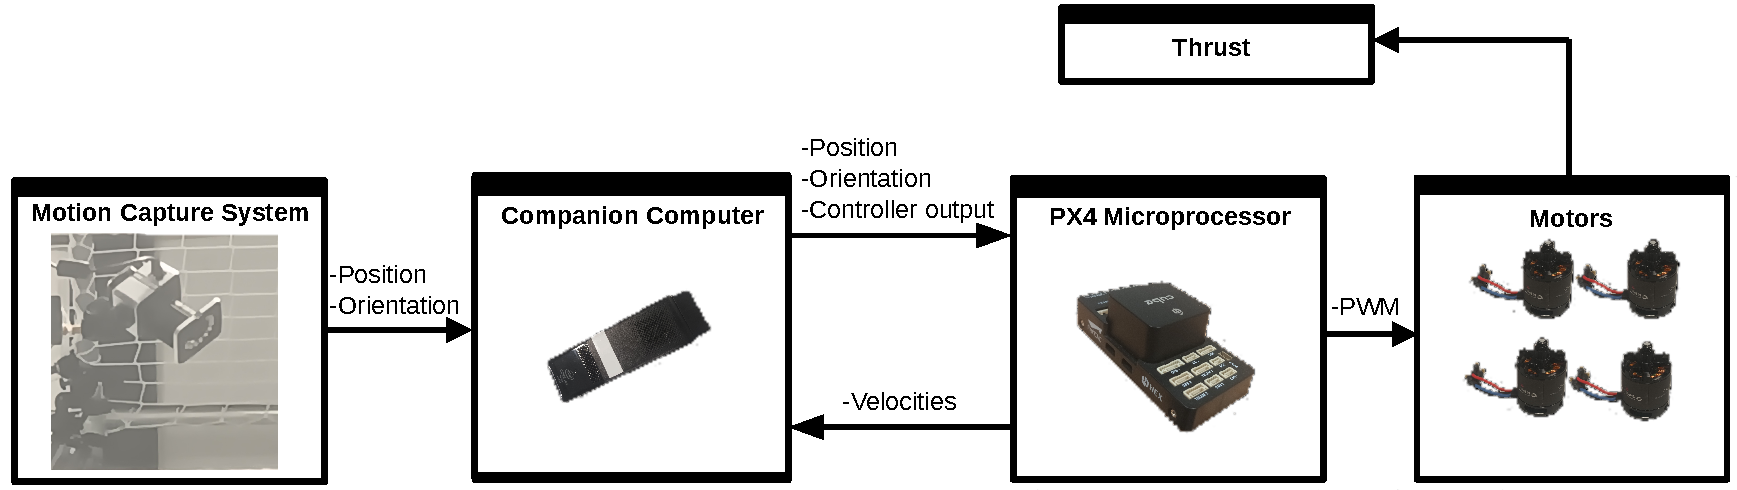
\includegraphics[width=1.0\linewidth]{figures/Deployment_figure.pdf}
    \caption{Real-world deployment of the generated control system onto a UAV with a motion capture system. The motion capture system sends precise position and orientation information to the companion computer\DIFdelbeginFL \DIFdelFL{through a TCP connection in an ENU coordinate frame}\DIFdelendFL . The companion computer \DIFdelbeginFL \DIFdelFL{converts the ENU frame into a NED frame and publishes it to the PX4 board. The PX4 board }\DIFdelendFL sends \DIFdelbeginFL \DIFdelFL{vehicle odometry gathered from an Extended Kalman Filter (EKF) back to the companion computer, which subsequently sends }\DIFdelendFL body-torque and collective thrust commands to the \DIFdelbeginFL \DIFdelFL{microprocessor}\DIFdelendFL \DIFaddbeginFL \DIFaddFL{PX4 microcontroller}\DIFaddendFL . The \DIFdelbeginFL \DIFdelFL{microprocessor }\DIFdelendFL \DIFaddbeginFL \DIFaddFL{microcontroller }\DIFaddendFL performs control allocation to convert the normalised thrust commands into PWM commands and interfaces them to the motors.\DIFdelbeginFL \DIFdelFL{The motors produce thrust, which alters the forces acting on the UAV, thereby changing its position and orientation.}\DIFdelendFL }
    \label{fig:deployment_figure}
\end{figure*}

\begin{figure}[!h]
    \centering
    \includegraphics[width=\linewidth]{figures/px4_topics.pdf}
    \caption{\textbf{PX4-ROS 2 interation:} Interaction between PX4 and the ROS2 nodes via a publisher/subscriber design pattern.}
    \label{fig:control-system-block}
\end{figure}



\subsection{Software-in-the-loop (SITL) testing}
\DIFaddbegin \DIFadd{While it is possible to skip a custom simulator and use Gazebo directly to create controllers, it is not recommended. If a controller is `built' while using Gazebo as a training environment in an attempt for direct deployment (Gazebo to real world), a large risk of overfitting remains. We use Gazebo here as the second environment to check for overfitting and confirm the control systems can interpolate information within new, unseen environments.
}

\DIFaddend As the generated controller produced acceptable results in the training environment, we prepared the algorithm for real-world deployment by transitioning it into a ROS 2 node that interfaces with PX4. PX4 enables SITL testing before deployment with high-fidelity simulations that integrate seamlessly into PX4 firmware. The SITL simulations offer a form of OOD testing and are higher quality and offer more insight into actual UAV performance than our training environment \cite{carr2024simulation, 10974379}.

The ROS2 node was integrated into PX4 Autopilot using the Micro-XRCE-DDS bridge. PX4 utilises a publisher/subscriber design pattern to exchange information between the onboard flight controller and an offboard controller. This integration allows us to treat the generated controller as a part of the PX4 firmware, benefiting from low-latency communication and access to internal state estimations. The generated controller, as a ROS 2 node, required some minor implementation changes before it functioned as intended. PX4 requires that the controller output is both normalised relative to the motor output and in a NED world frame. The generated controller, as designed, outputs absolute torque and thrust values (N) in a FLU world frame. We send the thrust and torque commands to PX4 at a rate of 8ms, with the controller receiving sensor updates at the same rate. 

A diagram illustrating the interaction between the generated controller and PX4 via PX4 topics is shown in Figure \ref{fig:control-system-block}.

\DIFdelbegin %DIFDELCMD < \begin{figure*}[!ht]
%DIFDELCMD < %%%
\DIFdelendFL \DIFaddbeginFL \begin{figure*}[!tb]
\DIFaddendFL \centering
\DIFaddbeginFL \setlength{\tabcolsep}{2pt}
\renewcommand{\arraystretch}{0}
%DIF >  Note, generated this solution for figure placement
%DIF >  Target height per panel (tune 0.22–0.24 if needed)
\newcommand{\panelH}{0.165\textheight}
\DIFaddendFL 

%DIF < -------------------- SITL --------------------
\DIFdelbeginFL %DIFDELCMD < \begin{minipage}{0.32\textwidth}
%DIFDELCMD <     \includegraphics[width=\linewidth]{figures/pid_dob_rvolmea_lemniscate_x.pdf}
%DIFDELCMD <     \caption*{Px error, lemniscate trajectory (SITL)}
%DIFDELCMD <     \label{fig:px_sitl}
%DIFDELCMD < \end{minipage}\hfill
%DIFDELCMD < \begin{minipage}{0.32\textwidth}
%DIFDELCMD <     \includegraphics[width=\linewidth]{figures/pid_dob_rvolmea_lemniscate_y.pdf}
%DIFDELCMD <     \caption*{Py error, lemniscate trajectory (SITL)}
%DIFDELCMD <     \label{fig:py_sitl}
%DIFDELCMD < \end{minipage}\hfill
%DIFDELCMD < \begin{minipage}{0.32\textwidth}
%DIFDELCMD <     \includegraphics[width=\linewidth]{figures/pid_dob_rvolmea_lemniscate_z.pdf}
%DIFDELCMD <     \caption*{Pz error, lemniscate trajectory (SITL)}
%DIFDELCMD <     \label{fig:pz_sitl}
%DIFDELCMD < \end{minipage}
%DIFDELCMD < \begin{minipage}{0.32\textwidth}
%DIFDELCMD <     \includegraphics[width=\linewidth]{figures/lissajous_sitl_x.pdf}
%DIFDELCMD <     \caption*{Px error, Lissajous trajectory (SITL)}
%DIFDELCMD <     \label{fig:pxl_sitl}
%DIFDELCMD < \end{minipage}\hfill
%DIFDELCMD < \begin{minipage}{0.32\textwidth}
%DIFDELCMD <     \includegraphics[width=\linewidth]{figures/lissajous_sitl_y.pdf}
%DIFDELCMD <     \caption*{Py error, Lissajous trajectory (SITL)}
%DIFDELCMD <     \label{fig:pyl_sitl}
%DIFDELCMD < \end{minipage}\hfill
%DIFDELCMD < \begin{minipage}{0.32\textwidth}
%DIFDELCMD <     \includegraphics[width=\linewidth]{figures/lissajous_sitl_z.pdf}
%DIFDELCMD <     \caption*{Pz error, Lissajous trajectory (SITL)}
%DIFDELCMD <     \label{fig:pzl_sitl}
%DIFDELCMD < \end{minipage}
%DIFDELCMD < \vspace{1.2em}
%DIFDELCMD < %%%
\DIFdelendFL \DIFaddbeginFL \begin{tabular}{@{}c c c@{}}
\DIFaddendFL 

%DIF < -------------------- REAL WORLD --------------------
\DIFdelbeginFL %DIFDELCMD < \begin{minipage}[!htb]{0.32\textwidth}
%DIFDELCMD <     \includegraphics[width=\linewidth]{figures/pid_dob_rvolmea_lemniscate_x_real.pdf}
%DIFDELCMD <     \caption*{Px error, lemniscate trajectory (Real-world)}
%DIFDELCMD <     \label{fig:px_real}
%DIFDELCMD < \end{minipage}\hfill
%DIFDELCMD < \begin{minipage}{0.32\textwidth}
%DIFDELCMD <     \includegraphics[width=\linewidth]{figures/pid_dob_rvolmea_lemniscate_y_real.pdf}
%DIFDELCMD <     \caption*{Py error, lemniscate trajectory (Real-world)}
%DIFDELCMD <     \label{fig:py_real}
%DIFDELCMD < \end{minipage}\hfill
%DIFDELCMD < \begin{minipage}{0.32\textwidth}
%DIFDELCMD <     \includegraphics[width=\linewidth]{figures/pid_dob_rvolmea_lemniscate_z_real.pdf}
%DIFDELCMD <     \caption*{Pz error, lemniscate trajectory (Real-world)}
%DIFDELCMD <     \label{fig:pz_real}
%DIFDELCMD < \end{minipage}
%DIFDELCMD < %%%
\DIFdelendFL \DIFaddbeginFL \subfloat[$P_x$ error, Lemniscate (SITL)\label{fig:lem_sitl_x}]%DIF > 
{\includegraphics[height=\panelH,width=0.32\textwidth]{figures/pid_dob_rvolmea_lemniscate_x.pdf}} &
\subfloat[$P_y$ error, Lemniscate (SITL)\label{fig:lem_sitl_y}]%DIF > 
{\includegraphics[height=\panelH,width=0.32\textwidth]{figures/pid_dob_rvolmea_lemniscate_y.pdf}} &
\subfloat[$P_z$ error, Lemniscate (SITL)\label{fig:lem_sitl_z}]%DIF > 
{\includegraphics[height=\panelH,width=0.32\textwidth]{figures/pid_dob_rvolmea_lemniscate_z.pdf}} \\[-1pt]
\DIFaddendFL 

\DIFdelbeginFL %DIFDELCMD < \begin{minipage}{0.32\textwidth}
%DIFDELCMD <     \includegraphics[width=\linewidth]{figures/lissajous_real_x.pdf}
%DIFDELCMD <     \caption*{Px error, Lissajous trajectory (Real-world)}
%DIFDELCMD <     \label{fig:px_real}
%DIFDELCMD < \end{minipage}\hfill
%DIFDELCMD < \begin{minipage}{0.32\textwidth}
%DIFDELCMD <     \includegraphics[width=\linewidth]{figures/lissajous_real_y.pdf}
%DIFDELCMD <     \caption*{Py error, Lissajous trajectory (Real-world)}
%DIFDELCMD <     \label{fig:py_real}
%DIFDELCMD < \end{minipage}\hfill
%DIFDELCMD < \begin{minipage}{0.32\textwidth}
%DIFDELCMD <     \includegraphics[width=\linewidth]{figures/lissajous_real_z.pdf}
%DIFDELCMD <     \caption*{Pz error, Lissajous trajectory (Real-world)}
%DIFDELCMD <     \label{fig:pz_real}
%DIFDELCMD < \end{minipage}
%DIFDELCMD < %%%
\DIFdelendFL \DIFaddbeginFL \subfloat[$P_x$ error, Lissajous (SITL)\label{fig:liss_sitl_x}]%DIF > 
{\includegraphics[height=\panelH,width=0.32\textwidth]{figures/lissajous_sitl_x.pdf}} &
\subfloat[$P_y$ error, Lissajous (SITL)\label{fig:liss_sitl_y}]%DIF > 
{\includegraphics[height=\panelH,width=0.32\textwidth]{figures/lissajous_sitl_y.pdf}} &
\subfloat[$P_z$ error, Lissajous (SITL)\label{fig:liss_sitl_z}]%DIF > 
{\includegraphics[height=\panelH,width=0.32\textwidth]{figures/lissajous_sitl_z.pdf}} \\[4pt]
\DIFaddendFL 

\DIFaddbeginFL \subfloat[$P_x$ error, Lemniscate (Real-world)\label{fig:lem_real_x}]%DIF > 
{\includegraphics[height=\panelH,width=0.32\textwidth]{figures/pid_dob_rvolmea_lemniscate_x_real.pdf}} &
\subfloat[$P_y$ error, Lemniscate (Real-world)\label{fig:lem_real_y}]%DIF > 
{\includegraphics[height=\panelH,width=0.32\textwidth]{figures/pid_dob_rvolmea_lemniscate_y_real.pdf}} &
\subfloat[$P_z$ error, Lemniscate (Real-world)\label{fig:lem_real_z}]%DIF > 
{\includegraphics[height=\panelH,width=0.32\textwidth]{figures/pid_dob_rvolmea_lemniscate_z_real.pdf}} \\[-1pt]

\subfloat[$P_x$ error, Lissajous (Real-world)\label{fig:liss_real_x}]%DIF > 
{\includegraphics[height=\panelH,width=0.32\textwidth]{figures/lissajous_real_x.pdf}} &
\subfloat[$P_y$ error, Lissajous (Real-world)\label{fig:liss_real_y}]%DIF > 
{\includegraphics[height=\panelH,width=0.32\textwidth]{figures/lissajous_real_y.pdf}} &
\subfloat[$P_z$ error, Lissajous (Real-world)\label{fig:liss_real_z}]%DIF > 
{\includegraphics[height=\panelH,width=0.32\textwidth]{figures/lissajous_real_z.pdf}} \\

\end{tabular}

\vspace{0.5em}

\DIFaddendFL \caption{\DIFdelbeginFL \textbf{\DIFdelFL{Results: }}%DIFAUXCMD
\DIFdelendFL \DIFaddbeginFL \textbf{\DIFaddFL{Results:}} \DIFaddendFL Comparison of SITL and real-world tracking errors for the \DIFdelbeginFL \DIFdelFL{lemniscate }\DIFdelendFL \DIFaddbeginFL \DIFaddFL{Lemniscate }\DIFaddendFL and Lissajous trajectories. \DIFdelbeginFL \DIFdelFL{The label }\DIFdelendFL RVOLMEA \DIFdelbeginFL \DIFdelFL{is used to identify }\DIFdelendFL \DIFaddbeginFL \DIFaddFL{denotes }\DIFaddendFL the generated \DIFdelbeginFL \DIFdelFL{control system}\DIFdelendFL \DIFaddbeginFL \DIFaddFL{controller}\DIFaddendFL . \DIFdelbeginFL \DIFdelFL{Variation between SITL and real-world results is expected, given the change in environments. Consistent with the existing literature, the SITL results are closer to real-world results than those from the training environment. The figures }\DIFdelendFL \DIFaddbeginFL \DIFaddFL{Subfigures (a)–(l) }\DIFaddendFL show \DIFdelbeginFL \DIFdelFL{the reference }\DIFdelendFL \DIFaddbeginFL \DIFaddFL{axis-wise tracking }\DIFaddendFL error over time for the best lap \DIFdelbeginFL \DIFdelFL{of any given controller }\DIFdelendFL (\DIFdelbeginFL \DIFdelFL{the }\DIFdelendFL lowest MSE\DIFdelbeginFL \DIFdelFL{lap}\DIFdelendFL ).}
\label{fig:lemniscate_fullpage}
\end{figure*}




\begin{table}[h!]
    \centering
    \caption{Per-lap Performance Metrics Comparison SITL}
    \label{tab:performance_metrics_sitl}
    \begin{tabular}{|c|c|c|c|}
        \hline
        \textbf{Controller} & \textbf{MSE} & \textbf{Std. dev} & \textbf{Best MSE} \\ \hline

        \multicolumn{4}{|c|}{\textbf{Lemniscate (SITL)}} \\ \hline
        Generated Controller & \textbf{0.0304$m^2$} & 0.0031$m^2$ & \textbf{0.0245$m^2$} \\ \hline
        PID+DOB & 0.0418$m^2$ & \textbf{0.0012$m^2$} & 0.0393$m^2$ \\ \hline
        LQR & 0.0533$m^2$ & 0.0143$m^2$ & 0.0744$m^2$ \\ \hline

        \multicolumn{4}{|c|}{\textbf{Lissajous (SITL)}} \\ \hline
        % Add rows for Lemniscate here
        % Example:
        Generated Controller & \textbf{0.0084$m^2$} & \textbf{0.0006$m^2$} & \textbf{0.0071$m^2$} \\ \hline
        PID+DOB & 0.0107$m^2$ & 0.0008$m^2$ & 0.0088$m^2$ \\ \hline
        LQR & 0.0116$m^2$ & 0.0017$m^2$ & 0.0090$m^2$ \\ \hline
    \end{tabular}
\end{table}


Table \ref{tab:performance_metrics_sitl} quantitatively summarises the results of 10 laps in the SITL testing environment for both the lemniscate and Lissajous trajectories. 

\DIFaddbegin \begin{table}[h!]
    \centering
    \caption{\DIFaddFL{Per-lap Performance Metrics Comparison SITL}}
    \label{tab:classic_metrics}
    \begin{tabular}{|c|c|c|c|}
    \hline
    \textbf{\DIFaddFL{Controller}} & \textbf{\DIFaddFL{Rise time}} & \textbf{\DIFaddFL{Settling time}} & \textbf{\DIFaddFL{$s$ error}} \\ \hline
    \DIFaddFL{Generated controller }& \DIFaddFL{1.296s }& \DIFaddFL{3.832s }& \DIFaddFL{0.003m }\\ \hline
    \DIFaddFL{PID+DOB }& \textbf{\DIFaddFL{0.776}}\DIFaddFL{s }& \textbf{\DIFaddFL{2.504}}\DIFaddFL{s}& \textbf{\DIFaddFL{0.001}}\DIFaddFL{m }\\ \hline
    \DIFaddFL{LQR }& \DIFaddFL{1.120s }& \DIFaddFL{2.792s }& \DIFaddFL{0.003m }\\ \hline
    \end{tabular}
\end{table}

\DIFadd{Additional SITL tests were performed to confirm the UAV control system's response against more classical metrics, summarised in Table \ref{tab:classic_metrics}. Note here that $s$ error refers to the steady state error of the UAV.
}

\DIFaddend On the lemniscate trajectory, the generated control system \DIFdelbegin \DIFdel{offered }\DIFdelend \DIFaddbegin \DIFadd{achieved }\DIFaddend a mean performance increase of 27.27\% \DIFdelbegin \DIFdel{compared to }\DIFdelend \DIFaddbegin \DIFadd{over }\DIFaddend the best-performing hand-made controller (PID+DOB). The worst lap of the generated control system outperformed the best lap of the PID+DOB control system. The reduced variance and standard deviation within laps of the PID+DOB control system are likely due to the DOB controller reaching its disturbance-estimation limits in the presence of model inaccuracies. For the generated control system, no disturbance observer or online model estimation is available, which contributes to \DIFdelbegin \DIFdel{the increased variation per lap}\DIFdelend \DIFaddbegin \DIFadd{increased lap-to-lap variation}\DIFaddend .

SITL results are displayed visually in Figure \ref{fig:lemniscate_fullpage}. \DIFaddbegin \DIFadd{In Figure \ref{fig:lemniscate_fullpage}, we can see that the generated controller offered substantial improvement across most axis within all tasks. In some areas, specifically $P_z$ error within the Lissajous task, we can see large inital error within the control system. Postulations for this are that the sliding window used by the control system did not correctly handle a large inital input disturabance by the Lissajous trajectory.
}\DIFaddend 


\section{Deployment and Real World Results}
\DIFaddbegin \DIFadd{Results are gathered using a UAV inside the Autonomous Systems lab at Loughborough University. We conducted 10 flight experiments for each controller, across both Lemniscate and Lissajous trajectories. During deployment, there was little variability within the results, and no failed flights. We took safety measures to ensure the control systems did not cause damage to the environment: a designated experiment area that the operator cannot enter during flight, the UAVs are suspended via a pulley system such that they cannot fall from height, a kill switch on the UAVs to immediately cut power, and finally a fallback to PX4 in-built flight control system if the offboard control system fails to send a heartbeat for 100ms.
}

\DIFaddend The UAV is built using a Holybro Pixhawk 6X, which houses and runs the PX4 firmware. A USB connecting the companion computer and flight controller are plugged into the Holybro Pixhawk 6X. For real-world deployment, instead of using the position and orientation information provided by the PX4 IMU, we use a VICON motion tracking system, which overrides the PX4-provided estimates.
The motion tracking system provides more accurate estimates of the UAV's position, velocity, and orientation.
Figure \ref{fig:deployment_figure} describes our deployment setup in a visual format\DIFaddbegin \DIFadd{, whereby each component is shown with relative outputs and inputs}\DIFaddend .



The results of the experiments for the real-world experiments are also visualised in Figure \ref{fig:lemniscate_fullpage}.
\begin{table}[h!]
    \centering
    \caption{Per-lap Performance Metrics Comparison Real world}
    \label{tab:performance_metrics_real_world}
    \begin{tabular}{|c|c|c|c|c|}
        \hline
        \textbf{Controller} & \textbf{MSE} & \textbf{Std. dev} & \textbf{Best MSE} \\ \hline
        \multicolumn{4}{|c|}{\textbf{Lemniscate (REAL WORLD)}} \\ \hline

        Generated Controller & \textbf{0.0098}$m^2$ & \textbf{0.0010}$m^2$ & \textbf{0.0090}$m^2$ \\ \hline
        PID+DOB & 0.0329$m^2$ & 0.0125$m^2$ & 0.0187$m^2$ \\ \hline
        LQR & 0.0261$m^2$ & 0.0028$m^2$ & 0.0201$m^2$ \\ \hline
        \multicolumn{4}{|c|}{\textbf{Lissajous (REAL WOLRD)}} \\ \hline
        Generated Controller & \textbf{0.0084}$m^2$ & \textbf{0.0006}$m^2$ & \textbf{0.0071}$m^2$ \\ \hline
        PID+DOB & 0.0116$m^2$ & 0.0008$m^2$ & 0.0088$m^2$ \\ \hline
        LQR & 0.0116$m^2$ & 0.0017$m^2$ & 0.0090$m^2$ \\ \hline
    \end{tabular}
\end{table}

\DIFdelbegin \DIFdel{A results Table for the real-world results is }\DIFdelend \DIFaddbegin \DIFadd{Results are }\DIFaddend provided in Table \ref{tab:performance_metrics_real_world}.  Within the results, the average is taken over 10 laps of the trajectory. `MSE' refers to the MSE of all laps, and `Best MSE' is the lap with the lowest MSE. The generated controller yielded strong results in the real world. An MSE of 0.0098 $ m^2$ precision within the lemniscate trajectory highlights the strengths of our methodology, whilst also showcasing areas for improvement. We specifically highlight the area for improvement in our results, namely, the direct deployment and iteration in the real world.

The generated controller exhibited greater robustness than the PID+DOB. All runs were performed across two charge cycles of a lithium-ion battery, with each run using approximately 20\% of the battery charge. We observe sensitivity to battery charge across runs in the PID+DOB controller. The achieved Z-axis component is reduced as the battery charge decreases. Unlike the PID+DOB controller, the generated control system shows no sensitivity to the charge, with the achieved accuracy remaining consistent throughout the experiments.

The achieved accuracy is higher for the generated control system than for the baseline controller. Across the X and Y axes.  The generated control system achieved close agreement with the target tracking across the Z-component throughout all experiments.

It is possible that both control systems can achieve better performance through real-world specific tuning. It is important to note that these results are obtained without any tuning in either SITL testing or the real world. The entire process is automatic: the gains for the control systems are determined using PSO within the training simulator.

\section{Conclusion}
In conclusion, we have designed and tested an LLM-synthesised control system using two simulators. The simulators showed that the generated control system is reliable for unmanned flight.

After testing the control system in the real world, we provide proof that generated code can be used in a Reinforcement Learning-esque fashion to create functional real-world code.


Because we used a training environment, the generated controllers are subject to the same limitations as reinforcement learning, such as overfitting to the training environment (known as the sim-to-real gap). We base this conclusion on a 3x reduction in performance from the training environment to the real world. Also notable is the lack of online parameter estimation for the generated control systems. The cause is primarily our methodology. No online parameter estimation is required, as PSO already optimises the model towards our known model parameters during the simulation.

The choice of our task, unmanned flight, reflects the growth and capabilities of LLMs to synthesise high-quality code across many queries.

This work opens the door to the application of agentic AI in engineering design and to the creation of many different control systems for the real world. Primarily, the following steps in this work are the creation of certified control systems, which can each be tested in the real world without the need for an intermediate testing environment.

\DIFaddbegin \DIFadd{For future works, there are two main directions of focus. Firstly, it will be interesting to see this work applied to general purpose robotics-based tasks. The work here is applied to a control system, though the task itself can be anything that is measured via an objective function. Secondly, the removal of PSO for other technqiues is a viable place for exploration. It will be interesting to see if evolution in the surrogate optimisation function over time, hand-in-hand with the primary candidate function, results in general improvement of the algorithm.
}

\DIFaddend Creating a methodology for unmanned flight is difficult. Simulated training environments are almost always required because poor control systems can lead to catastrophic failure in the real world. It would be interesting to apply this methodology directly to the real world, using online parameter estimation rather than PSO. This way, the limitations identified in this paper (overfitting and lack of generalisation) can be mitigated through real-world scoring and iteration. These control systems would need to be implemented on an unmanned vehicle, such as a TurtleBot, that is not in any intrinsic danger, so that faulty control systems can be easily discarded without damaging the machine executing them.
A link for viewing the \DIFdelbegin \DIFdel{implementation of all controllers with the lemniscate trajectory is provided }\href{https://github.com/jynxmagic/Px4-offboard-controllers-thrust-and-torque}{\DIFdel{here}}%DIFAUXCMD
\DIFdel{. The generated control system can be found under the function `rvolmeaControl'}\DIFdelend \DIFaddbegin \DIFadd{code used to generate the control system and deploy the control system to the UAV is provided in the references \mbox{%DIFAUXCMD
\cite{jynxmagic_generated_controller_ros2_2026}}\hskip0pt%DIFAUXCMD
}\DIFaddend .

% \subsection{Future works}
% Lorem ipsum dolor sit amet, consectetur adipiscing elit. Praesent commodo cursus magna, vel scelerisque nisl consectetur et. Donec sed odio dui. Nulla vitae elit libero, a pharetra augue. Nullam id dolor id nibh ultricies vehicula ut id elit. Curabitur blandit tempus porttitor. Integer posuere erat a ante venenatis dapibus posuere velit aliquet. Aenean lacinia bibendum nulla sed consectetur.

\vspace{11pt}

% \bf{If you will not include a photo:}\vspace{-33pt}
% \begin{IEEEbiographynophoto}{John Doe}
% Use $\backslash${\tt{begin\{IEEEbiographynophoto\}}} and the author name as the argument, followed by the biography text.
% \end{IEEEbiographynophoto}

\bibliographystyle{unsrt}
\bibliography{main}

% \vfill

\end{document}


